\addcontentsline{toc}{chapter}{Appendices}

\chapter{Appendices}
    \newpage
    % The \appendix command resets the chapter counter, and changes the chapter numbering scheme to capital letters.
    \appendix
    
    \chapter{PCA Data Driven Surrogate Signal Extraction Methods for Dynamic PET Full Overview} \label{sec:pca_data_driven_surrogate_signal_extraction_methods_for_dynamic_pet_full_overview}
        \begin{figure}
            \centering
            
            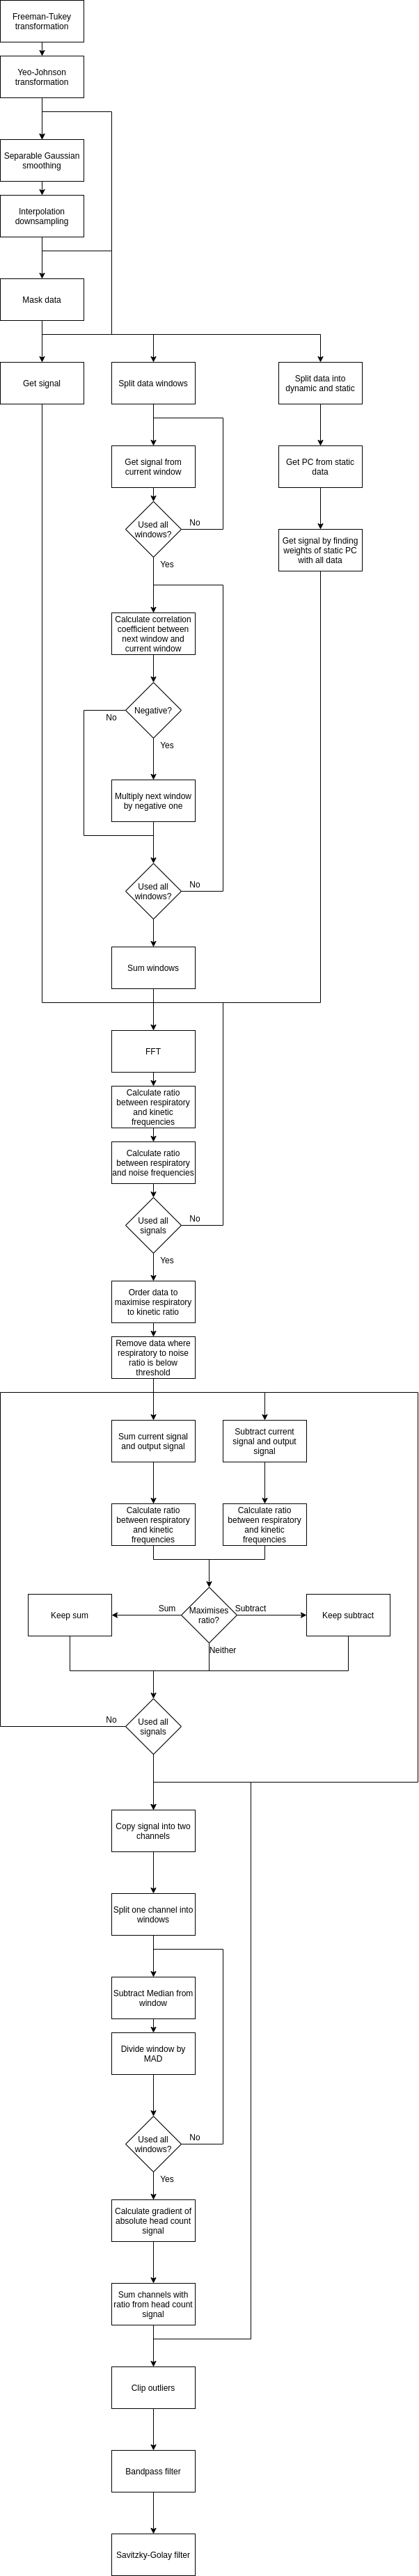
\includegraphics[width=0.2\linewidth]{figures/data_driven_surrogate_signal_extraction_methods_1_full_overview.png}
            
            \captionsetup{singlelinecheck=false, justification=centering}
            \caption{A diagram showing an overview of the possible ways in which the method could be executed.}
            \label{fig:pca_data_driven_surrogate_signal_extraction_methods_for_dynamic_pet_appendix_full_overview}
        \end{figure}
